\chapter{Laboratorio 4}
\begin{figure}[ht!]
	\centering
	\begin{minipage}{.45\textwidth}
		\scalebox{.62}{
			\begin{circuitikz}
				\draw (2,6) node[op amp, anchor=-](oa){\texttt{TL071}};
				\draw (oa.-) -- ++(-2, 0) coordinate (D) -- ++(-2,0) to[C=$C$] ++(0,-1.5) node[ground]{};
				\draw (D) to[D=$D$] ++(0,-1.5) node[ground]{};
				\draw (oa.up) -- ++(0, 0.3) node[vcc]{$V_{DD}$};
				\draw (oa.down) -- ++(0,-0.3) node[vee]{$V_{SS}$};
				\draw (oa.out) -- ++(1,0) coordinate(loop);
				\draw (loop) -- ++(0,-2.3) coordinate(R2) to[R=$R_2$] ++(-3.39,0) coordinate(rg) (R2-|oa.+) -- (oa.+);
				\draw (oa.-) -- ++(0,1.7) to[R=$R_3$]++(3.39,0) coordinate(Rf) (Rf-|loop) -- (loop);
				\draw (oa.+) to[short, -o] ++(0,0) ++(-.1,0) node[left]{$v_+$};
				\draw (oa.-) to[short, -o] ++(0,0) ++(0,-.1) node[below]{$v_-$};
				\draw (rg) -- ++(-1,0) coordinate(r1) to[R=$R_1$] ++(0,-2) node[ground]{};
				\draw (r1) to[D=$D_T$] ++(-2.5,0) coordinate(vt) to[C=$C_T$] ++(-3,0) coordinate(vin);
				\draw (vt) to[R=$R_T$] ++(0,-2) node[ground]{};
				\draw (vt) to[short, -o] ++(0,0) node[above]{$v_t$};
				\draw (loop) to[short, -o] ++(0,0) ++(.1,0) node[right]{$v_{out}$};
				\draw (vin) to[sV=$v_{in}$] ++(0,-2) node[ground]{};
				\draw[thick] (-5.5,0) rectangle (6.5,8.5);
			\end{circuitikz} 
		}
	\end{minipage}\qquad
	\begin{minipage}{.45\textwidth}
		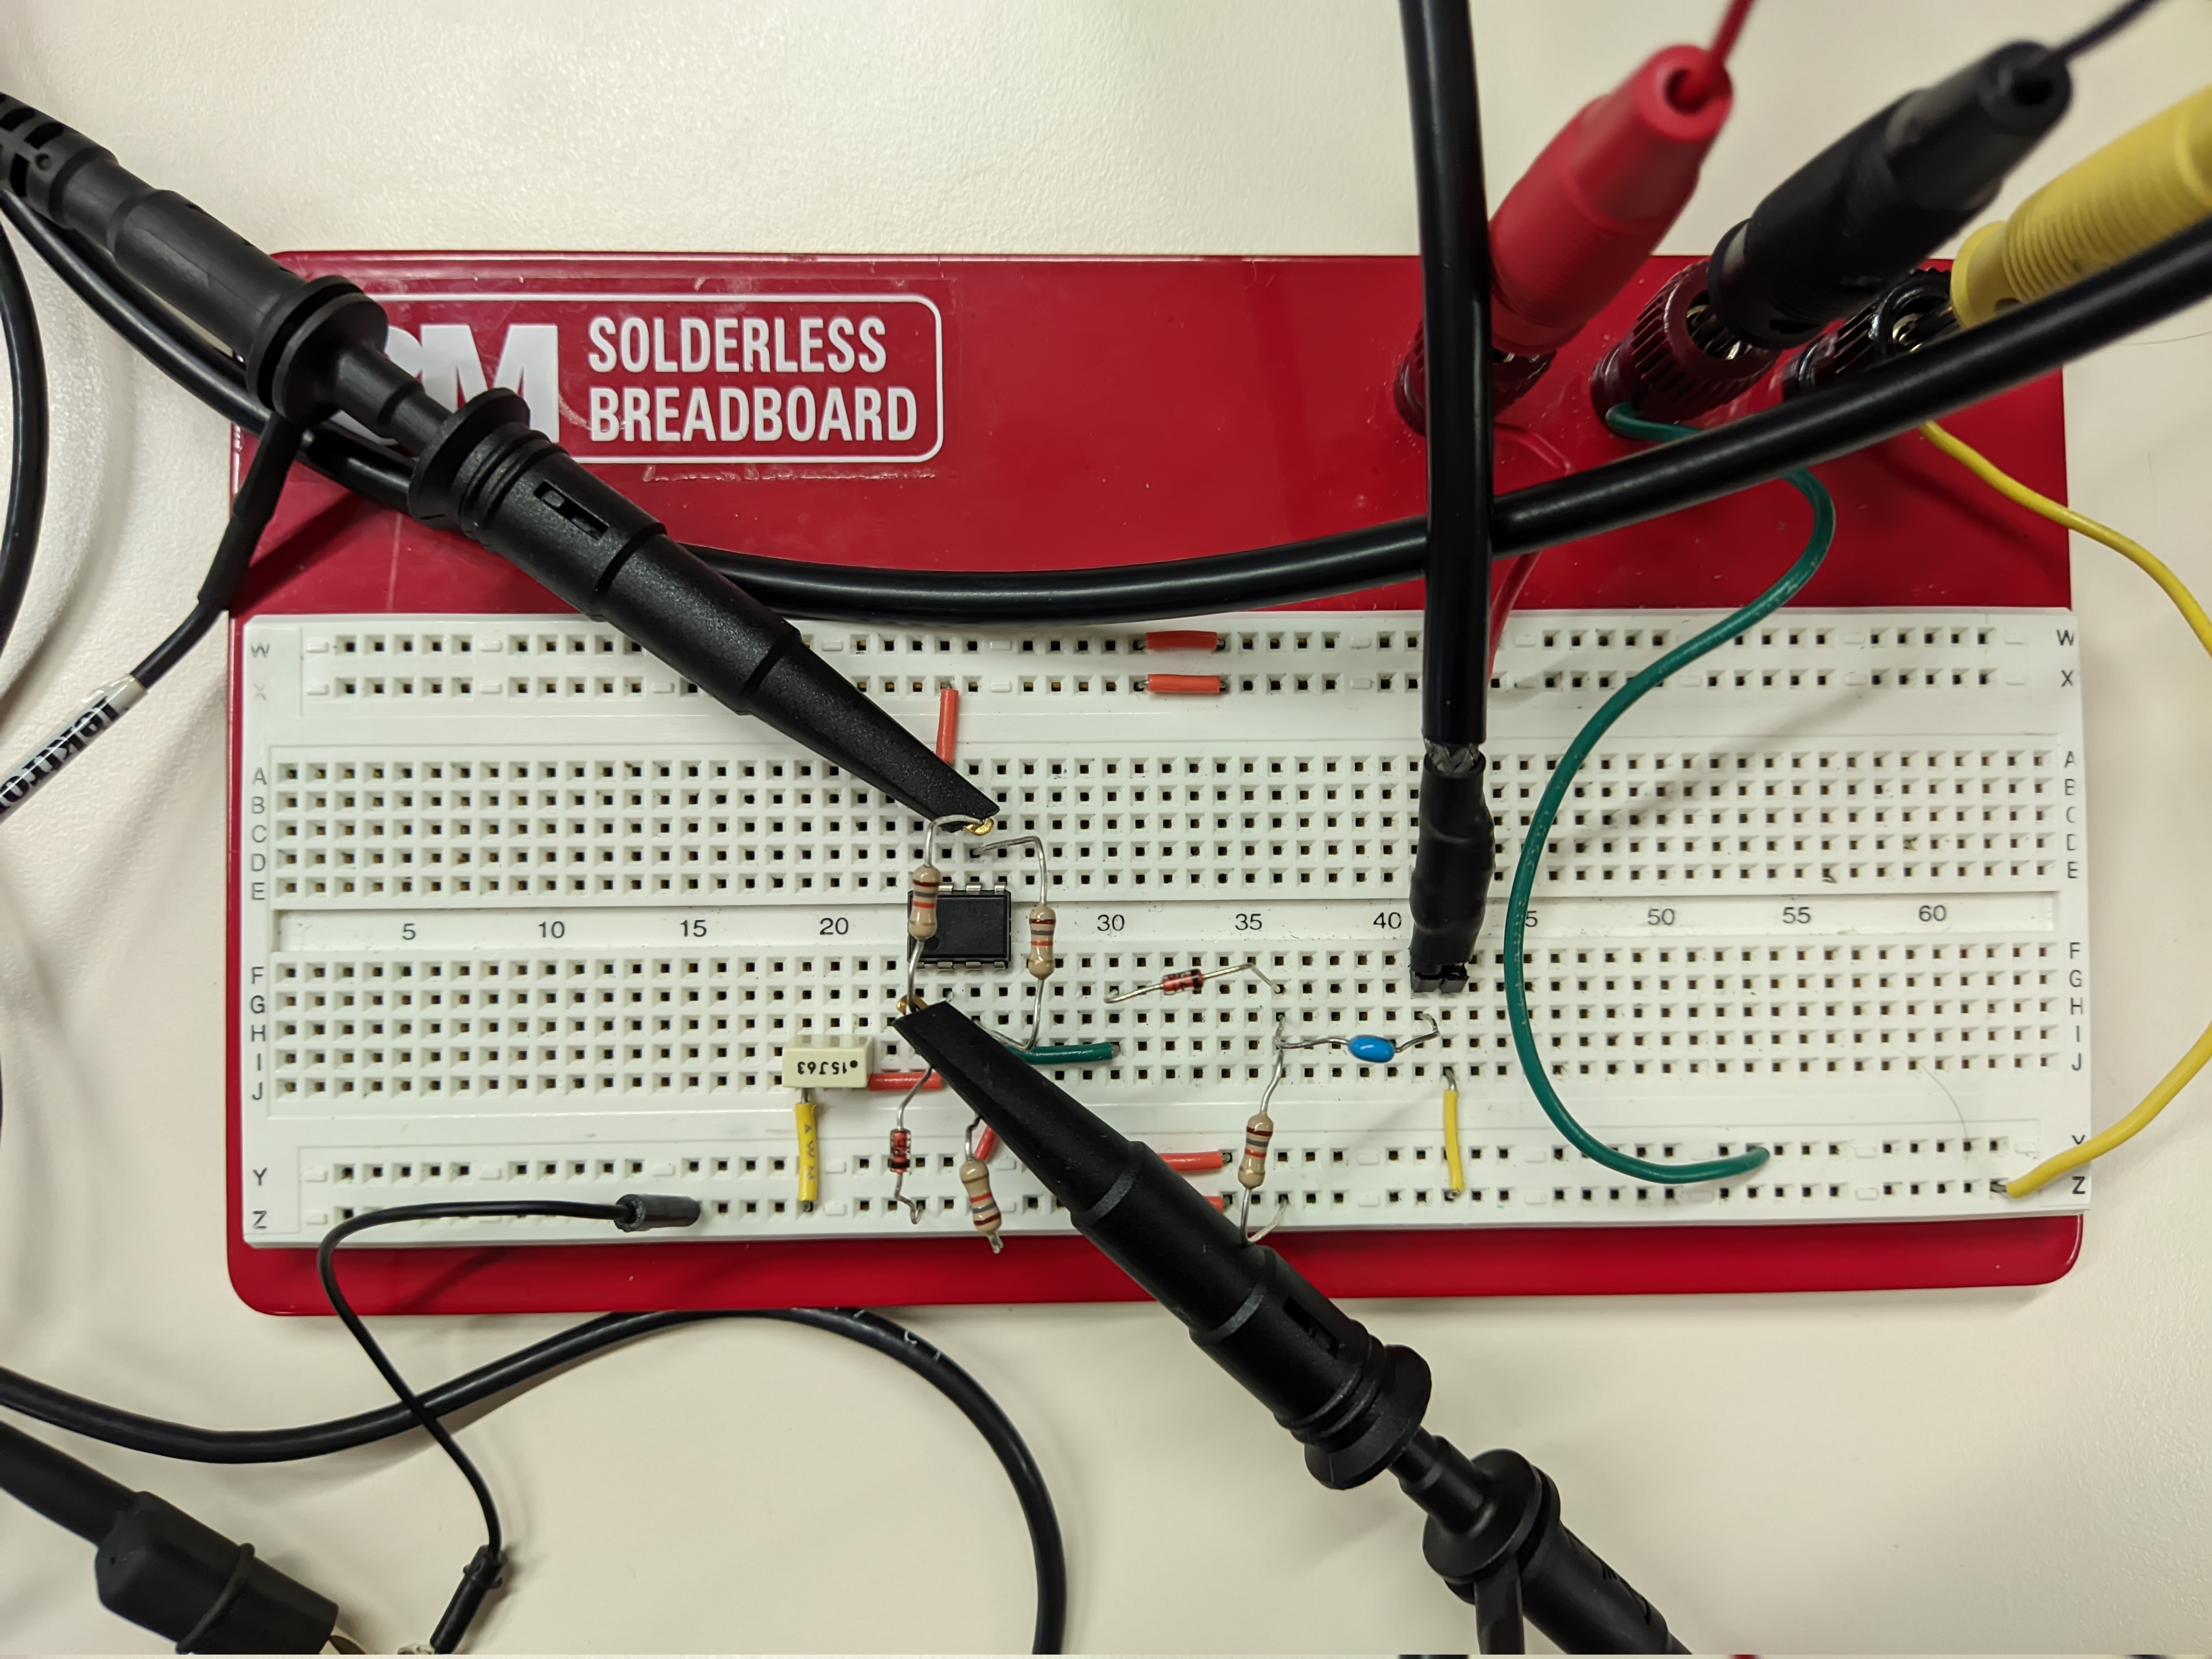
\includegraphics[width=\linewidth]{./ImageFiles/Laboratorio 4/CIR11.jpg}
	\end{minipage}
	\caption{Schema circuitale del circuito monostabile di precisione e foto del circuito realizzato.}
	\label{fig:circuito_1}
\end{figure}
Il primo circuito analizzato è un circuito monostabile, che a livello costruttivo è molto simile all'ultimo circuito della lezione precedente, con la differenza che questo non oscilla continuamente in base al rapporto tra le resistenze sull'operazionale \todo{Approfondire opportunamente questa sezione}, ma invece viene controllato tramite un opportuno segnale di ingresso. Questo segnale di ingresso causa il passaggio dallo stato stabile a quello non stabile, dove dopo un periodo di tempo configurato tramite la carica di una capacità, lo stesso ritorna nuovamente nello stato iniziale in attesa di un nuovo impulso fornito esternamente.

Lo stato stabile è forzato utilizzando un diodo messo in parallelo sulla capacità. Questo limita la tensione massima nella carica della stessa alla tensione di accensione del diodo $\approx 0,7$ invece che alla tensione di alimentazione $V_{cc}$ fornita all'amplificatore. Ciò impedisce la commutazione dell'op-amp se la tensione necessaria al morsetto $V_H^+$ è maggiore della caduta di tensione sul diodo. Questa si può calcolare come
\[V_H^+=\frac{R_1}{R_1+R_2}V_{DD}\overset{\mathrm{R_1=R_2}}=\frac{V_{DD}}{2}\]

I valori utilizzati nel nostro circuito sono indicati nella tabella \ref{tab:valori_componenti_1}. Inoltre, gli amplificatori sono stati alimentati con una tensione duale di $\pm$\SI{10}{\volt}.

\def\arraystretch{1.3}
\begin{table}[h]
	\centering
	\begin{tabular}{|c|c|c|}
		\hline
		Componente	& Valore Nominale & Valore Misurato \\ \hline
		R1 &\SI{18}{\kilo\ohm} & \SI{17,96}{\kilo\ohm} \\ \hline
		R2 &\SI{18}{\kilo\ohm} & \SI{17,79}{\kilo\ohm} \\ \hline
		R3 & \SI{18}{\kilo\ohm} & \SI{18}{\kilo\ohm} \\ \hline
		R\sub{T} & \SI{18}{\kilo\ohm} & \SI{17,83}{\kilo\ohm} \\ \hline
		D\sub{T} & $\simeq$\SI{0.7}{\volt} & \SI{609}{\milli\volt} \\ \hline
		D1 & $\simeq$\SI{0.7}{\volt} & \SI{607}{\milli\volt} \\ \hline
		C & \SI{150}{\nano\farad} & Non misurato \\ \hline
	\end{tabular}
	\caption{Valori nominali e misurati dei componenti utilizzati nel circuito.}
	\label{tab:valori_componenti_1}
\end{table}

Nel nostro caso specifico quindi $V_H^+ \approx \frac{V_{DD}}{2}\approx\SI{5}{\volt}>\SI{609}{\milli\volt}$. Questo quindi tiene il circuito stabile, visto che la capacità non potrà mai caricarsi oltre alla tensione di attivazione del diodo.

Per permettere la commutazione dell'op-amp si è aggiunta una seconda sezione del circuito sul morsetto positivo dell'operazionale, composta da un filtro RC e da un diodo.